\documentclass[conference]{IEEEtran}
\usepackage[utf8]{inputenc}
\usepackage[spanish,es-tabla]{babel}
\usepackage{graphicx}
\usepackage{amsmath, amssymb}
\usepackage{booktabs}
\usepackage{float}
\usepackage{url}

\begin{document}

\title{Análisis y Predicción de Precios Hoteleros en Río de Janeiro: Un Enfoque de Machine Learning}

\author{\IEEEauthorblockN{Narda Rosa}
\IEEEauthorblockA{\textit{Facultad de Ingeniería} \\
\textit{Universidad Austral}\\
Pilar, Argentina \\
nrosa@mail.austral.edu.ar}
\and
\IEEEauthorblockN{Julieta Kimel}
\IEEEauthorblockA{\textit{Facultad de Ingeniería} \\
\textit{Universidad Austral}\\
Pilar, Argentina \\
jkimel@mail.austral.edu.ar}}

\maketitle

\begin{abstract}
Este documento consolida el análisis exploratorio de datos (EDA) y la formulación de un modelo predictivo para estimar el precio por persona por noche en establecimientos hoteleros de Río de Janeiro. Se procesaron datos transaccionales de búsquedas, aislando factores geográficos, estacionales y de calidad. Tras corregir anomalías de integración y estabilizar métricas dispersas, se contrastó una regresión lineal paramétrica contra un algoritmo Random Forest. El ensamble no lineal demostró una capacidad explicativa superior, evidenciando que el mercado se rige primordialmente por la urgencia temporal y los monopolios de locación, relegando otros atributos de infraestructura a un rol secundario.
\end{abstract}

\begin{IEEEkeywords}
Machine Learning, Random Forest, EDA, Economía Espacial, Precios.
\end{IEEEkeywords}

\section{Integración y Estructura de los Datos}
El análisis comienza con la integración de dos conjuntos de datos principales:
\begin{itemize}
    \item \textbf{Searches (\texttt{searches\_6381}):} Contiene el historial de búsquedas de hoteles realizadas por los usuarios, incluyendo precios, fechas, características del hotel y si la búsqueda terminó en compra (\texttt{target}).
    \item \textbf{Amenities (\texttt{amenities\_descriptions}):} Un diccionario que mapea los códigos de las comodidades del hotel con su descripción en español.
\end{itemize}

\subsection{Proceso de Unión (Join)}
Se realizó un \texttt{left\_join} para cruzar la información. Es fundamental notar que al usar una variable indicadora binaria (como \texttt{amen\_ohe\_extraflag}) contra los códigos reales del diccionario, el cruce no encuentra coincidencias exactas. La decisión de usar un \texttt{left\_join} permitió preservar absolutamente todas las búsquedas originales, aunque explicó la altísima concentración de valores faltantes (NA) en las columnas descriptivas importadas.

\section{Análisis Exploratorio de Datos (EDA)}
El EDA revela patrones fundamentales sobre cómo los usuarios interactúan con la plataforma y cómo se estructuran los precios y valoraciones.

\subsection{Valores Faltantes}
Tras corregir la llave de integración entre los conjuntos de datos, el diagnóstico de completitud resulta sumamente favorable.

\begin{figure}[htbp]
    \centering
    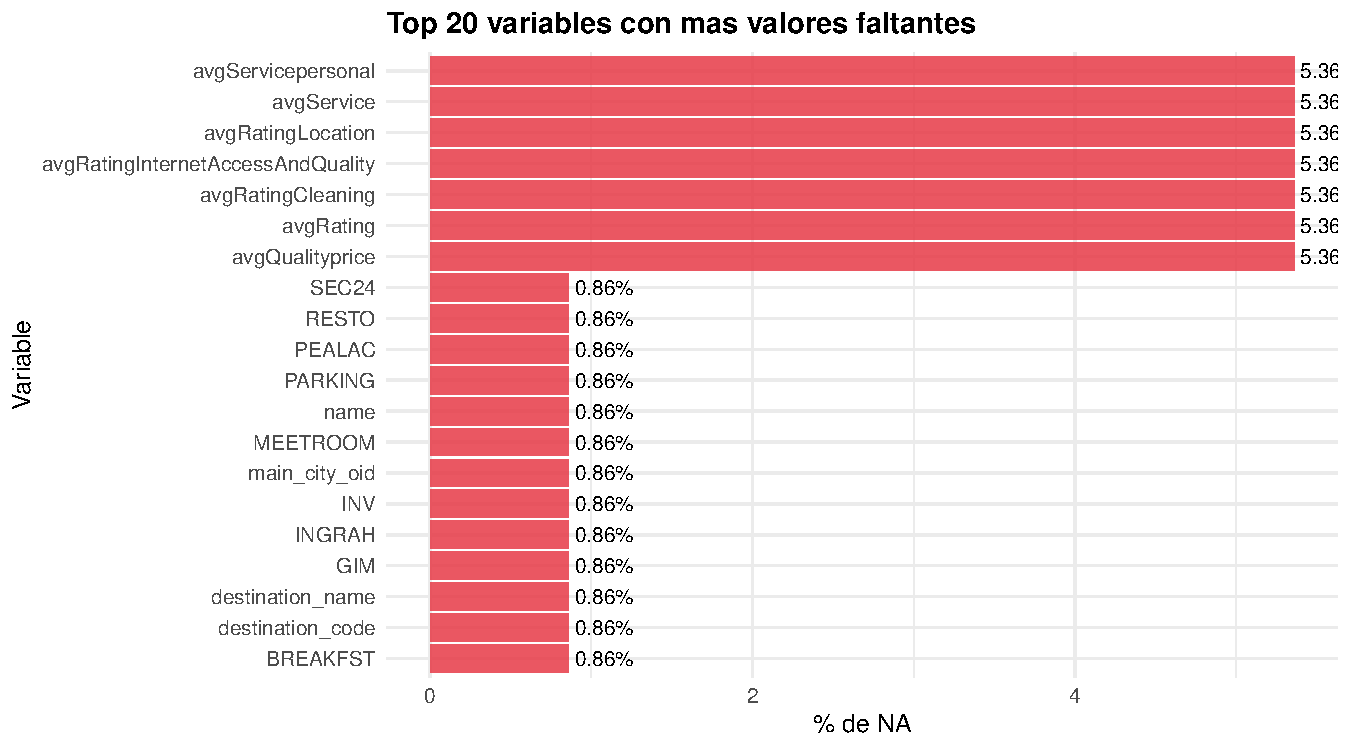
\includegraphics[width=\linewidth]{eda_nas_plot-1.pdf}
    \caption{Top 20 variables con más valores faltantes.}
\end{figure}

La mayor proporción de valores nulos recae exclusivamente en las variables de satisfacción y calificaciones por dimensión (como \texttt{avgServicepersonal} o \texttt{avgRatingLocation}), alcanzando apenas un 5.36\% de la muestra. Le siguen atributos binarios de infraestructura (\texttt{SEC24}, \texttt{PARKING}) con proporciones inferiores al 1\%. Al tratarse de valores marginales, se descarta la eliminación de columnas del espacio predictivo; la imputación de los ratings mediante la mediana condicionada resulta suficiente para retener la integridad de los datos.

\subsection{Distribución de la Variable Objetivo}
El gráfico de la variable \texttt{target} evidencia un fuerte desbalance de clases: el 95.68\% de las búsquedas no terminan en compra. 

\begin{figure}[htbp]
    \centering
    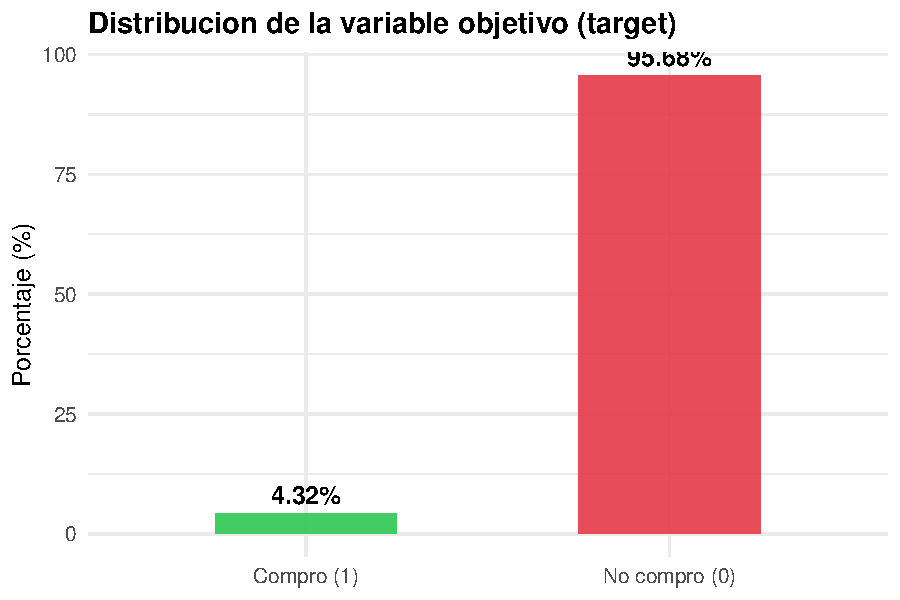
\includegraphics[width=\linewidth]{eda_target_plot-1.pdf}
    \caption{Distribución de la variable objetivo (Target).}
\end{figure}

Este patrón es típico en plataformas de viajes. Ignorarlo llevaría a modelos que predicen siempre ``0'' con alta exactitud (accuracy) pero sin utilidad real.

\subsection{Distribución del Precio}
La distribución presenta un fuerte sesgo positivo (cola a la derecha). La mayoría de los hoteles se concentra en un rango moderado, con algunos outliers de precio muy alto. La escala logarítmica es necesaria para visualizar correctamente esta asimetría.

\begin{figure}[htbp]
    \centering
    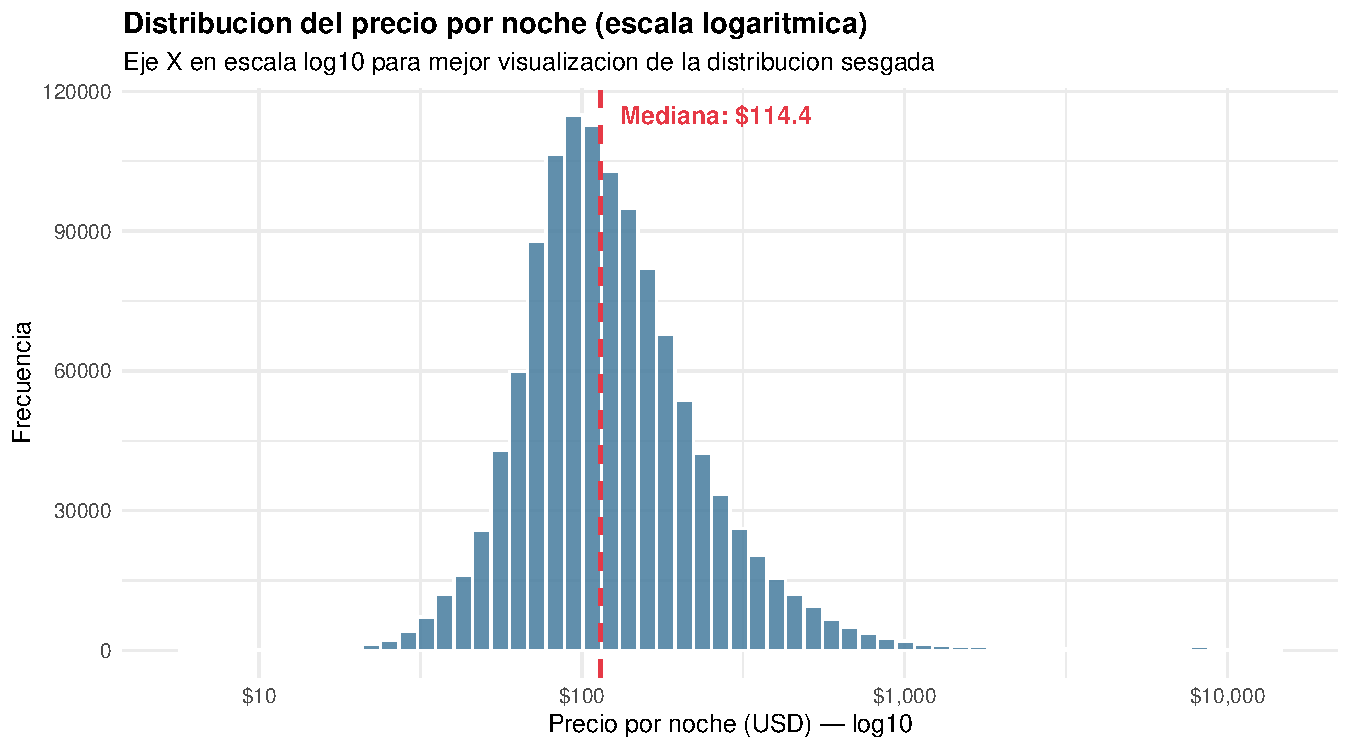
\includegraphics[width=\linewidth]{eda_precio_hist-1.pdf}
    \caption{Distribución del precio por noche (escala logarítmica).}
\end{figure}

Al segmentar el precio según si el usuario compró o no, observamos que los usuarios tienden a comprar hoteles dentro de un rango específico, lo que sugiere poder discriminativo.

\begin{figure}[htbp]
    \centering
    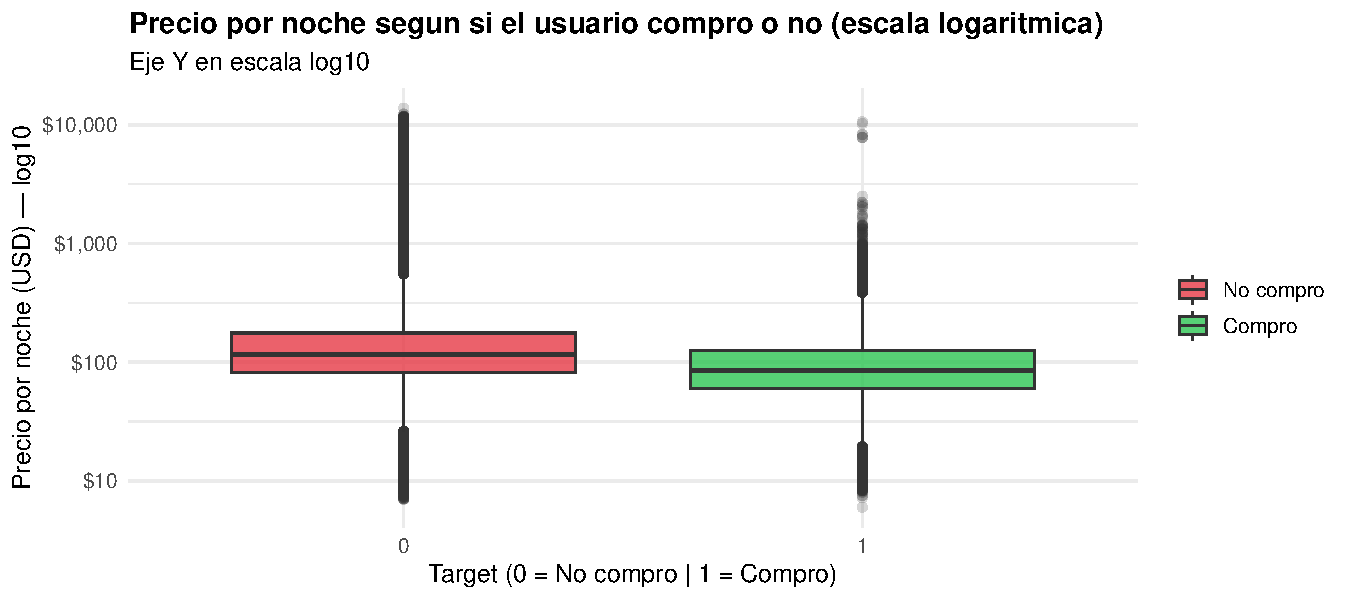
\includegraphics[width=\linewidth]{eda_precio_target-1.pdf}
    \caption{Precio por noche según target de compra.}
\end{figure}

\subsection{Categoría y Ratings}
La mayor parte de las búsquedas recae en hoteles de 3 y 4 estrellas, reflejando una preferencia por el segmento medio-alto. 

\begin{figure}[htbp]
    \centering
    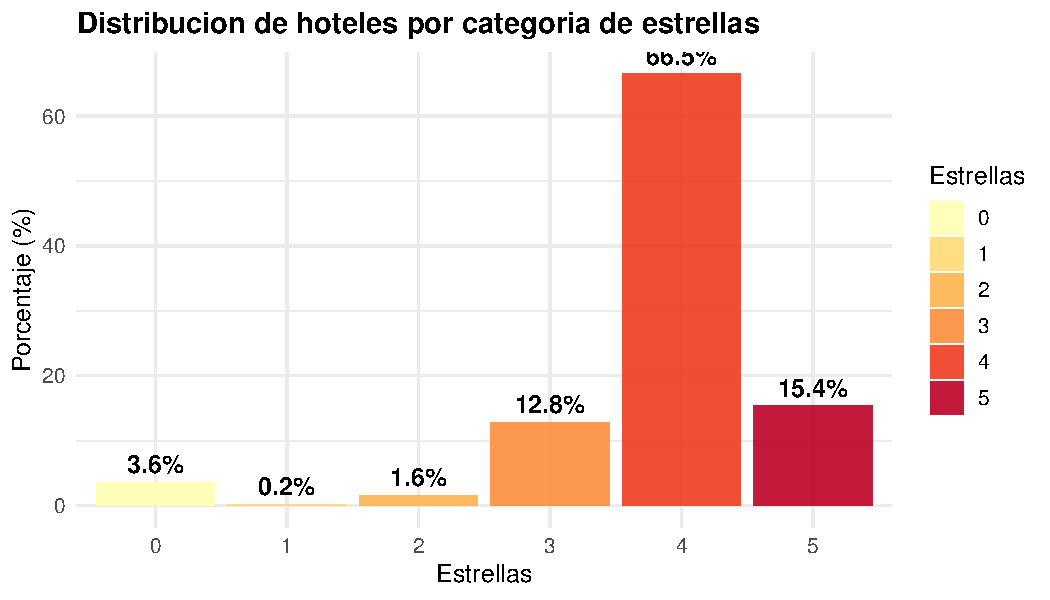
\includegraphics[width=\linewidth]{eda_estrellas-1.pdf}
    \caption{Distribución de hoteles por categoría de estrellas.}
\end{figure}

En cuanto a las dimensiones de satisfaction, la limpieza y la ubicación tienden a ser las mejor valoradas, mientras que \texttt{avgQualityprice} muestra mayor variabilidad de opiniones.

\begin{figure}[htbp]
    \centering
    \includegraphics[width=\linewidth]{eda_ratings_plot-1.pdf}
    \caption{Distribución de ratings por dimensión.}
\end{figure}

\subsection{Estacionalidad y Perfil de Usuario}
Brasil y Argentina dominan el volumen de búsquedas. Temporalmente, observamos una marcada estacionalidad con picos en enero, febrero (verano austral) y julio (vacaciones de invierno).

\begin{figure}[htbp]
    \centering
    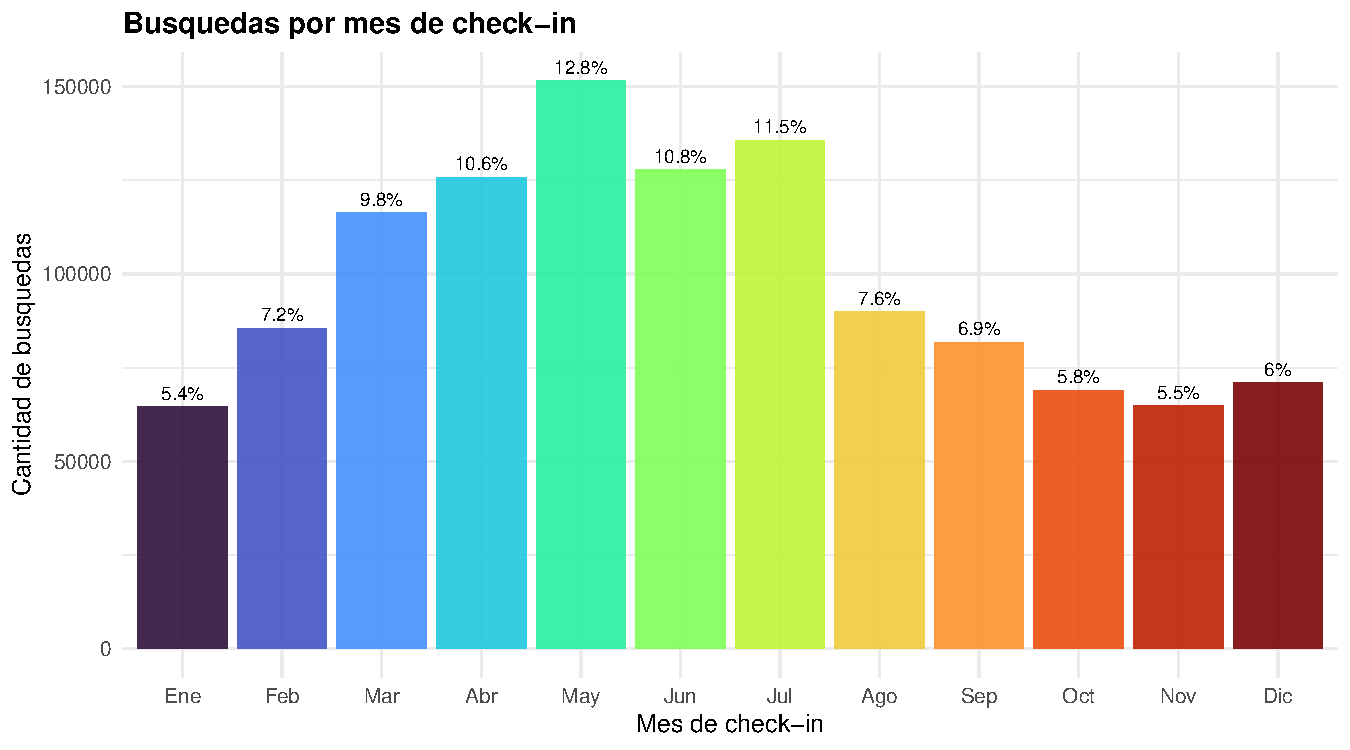
\includegraphics[width=\linewidth]{eda_mes_ci-1.pdf}
    \caption{Búsquedas por mes de check-in (Estacionalidad).}
\end{figure}

En términos de comportamiento, la anticipación revela dos perfiles: planificadores (semanas/meses) e impulsivos (1 a 7 días). Las estadías más frecuentes se concentran entre 1 y 3 noches.

\begin{figure}[htbp]
    \centering
    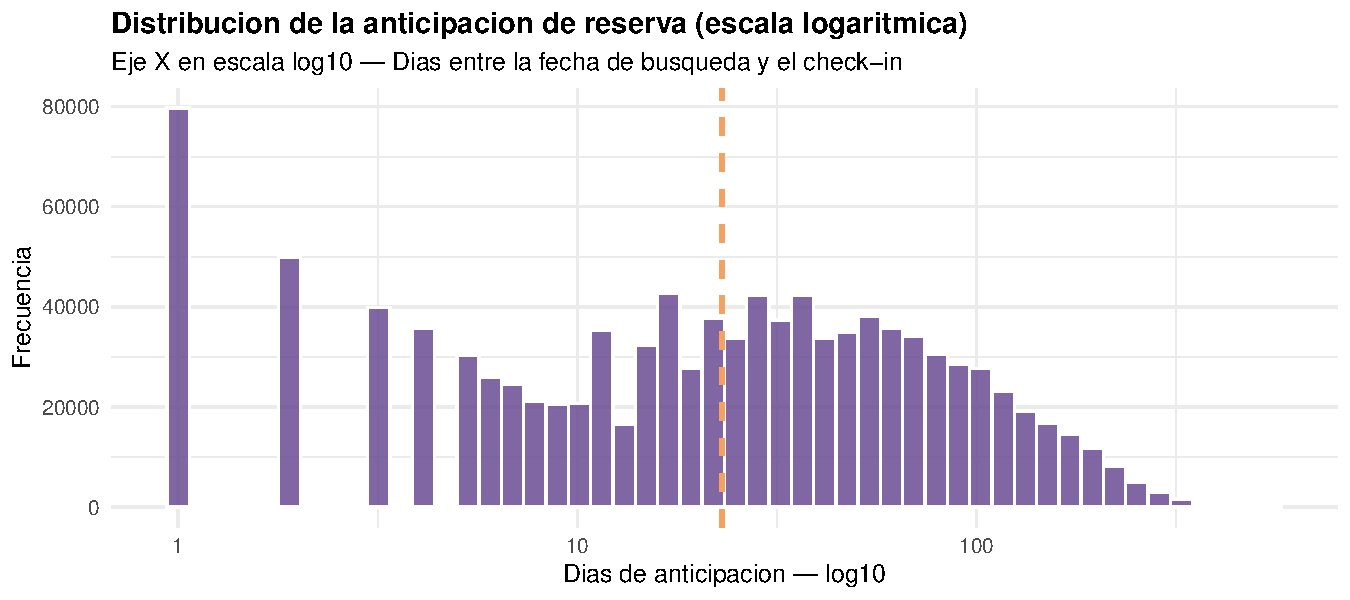
\includegraphics[width=\linewidth]{eda_anticipacion-1.pdf}
    \caption{Distribución de la anticipación de reserva.}
\end{figure}

\subsection{Correlaciones y Visibilidad}
La matriz de correlación evidencia que los diversos tipos de precio están fuertemente ligados entre sí, pero tienen baja relación lineal directa con el \texttt{target}. 

\begin{figure}[htbp]
    \centering
    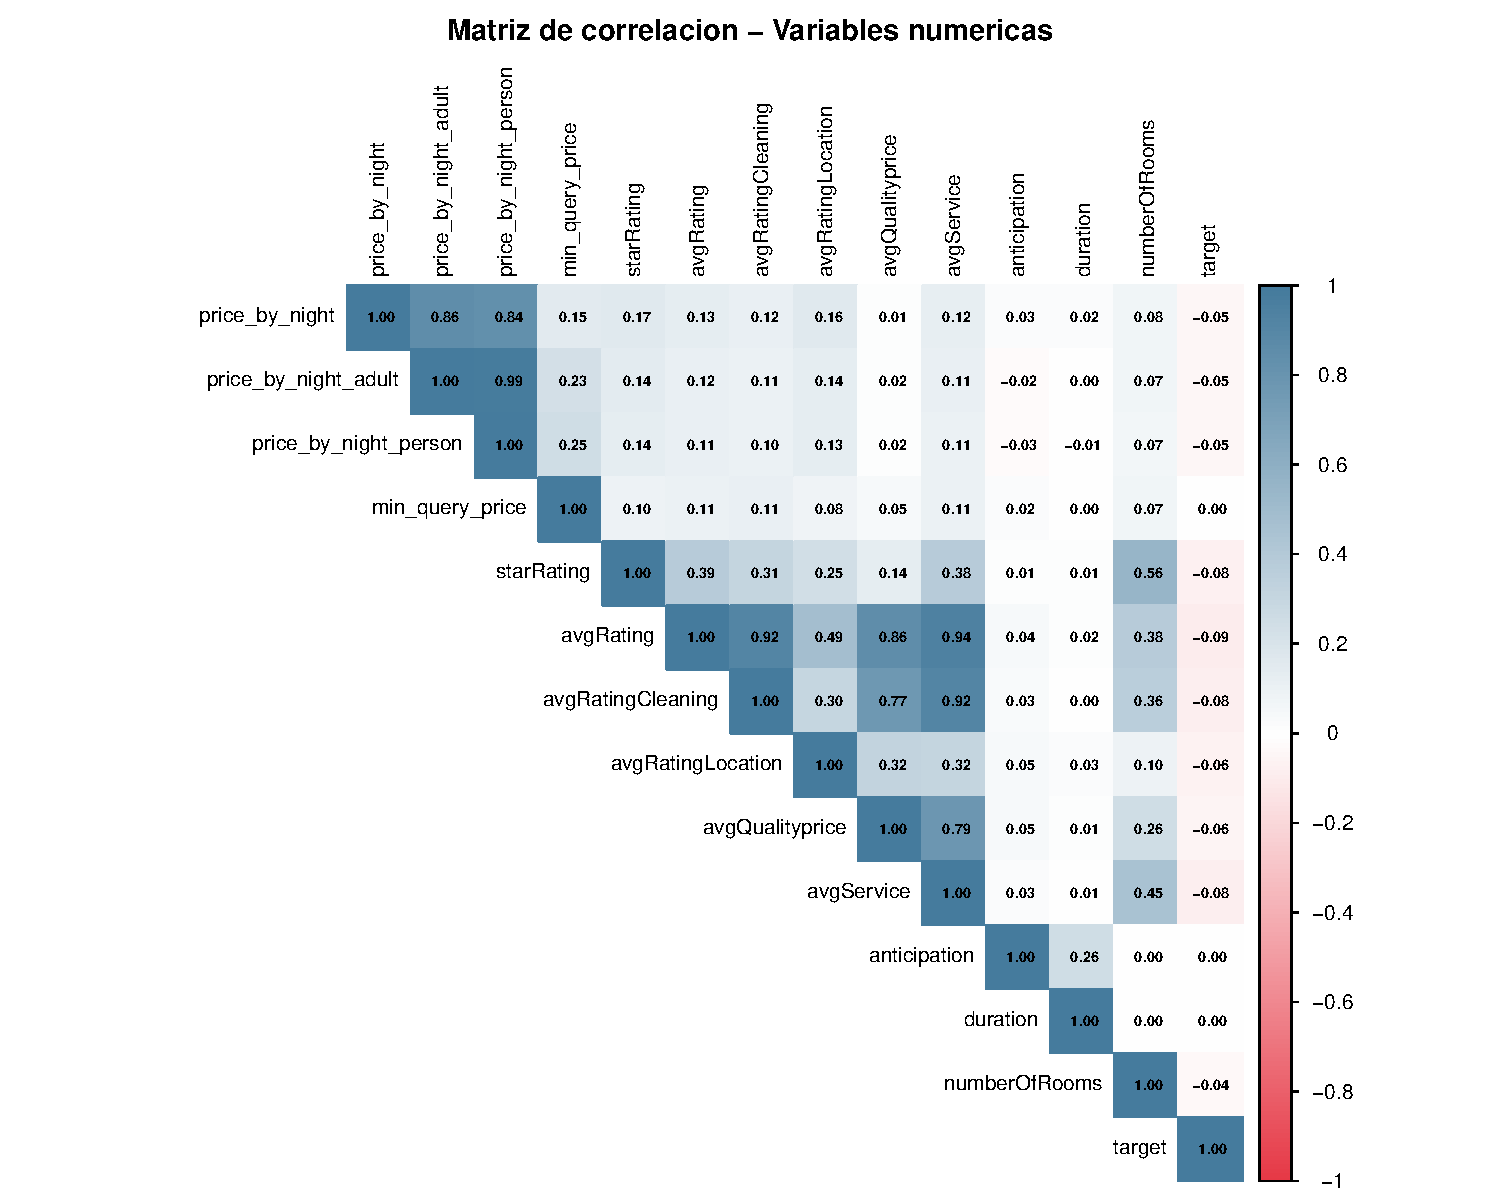
\includegraphics[width=\linewidth]{eda_correlacion-1.pdf}
    \caption{Matriz de correlación de variables numéricas.}
\end{figure}

Por otro lado, la posición en los resultados muestra un claro sesgo de visibilidad: las primeras posiciones acaparan la abrumadora mayoría de la conversión.

\begin{figure}[htbp]
    \centering
    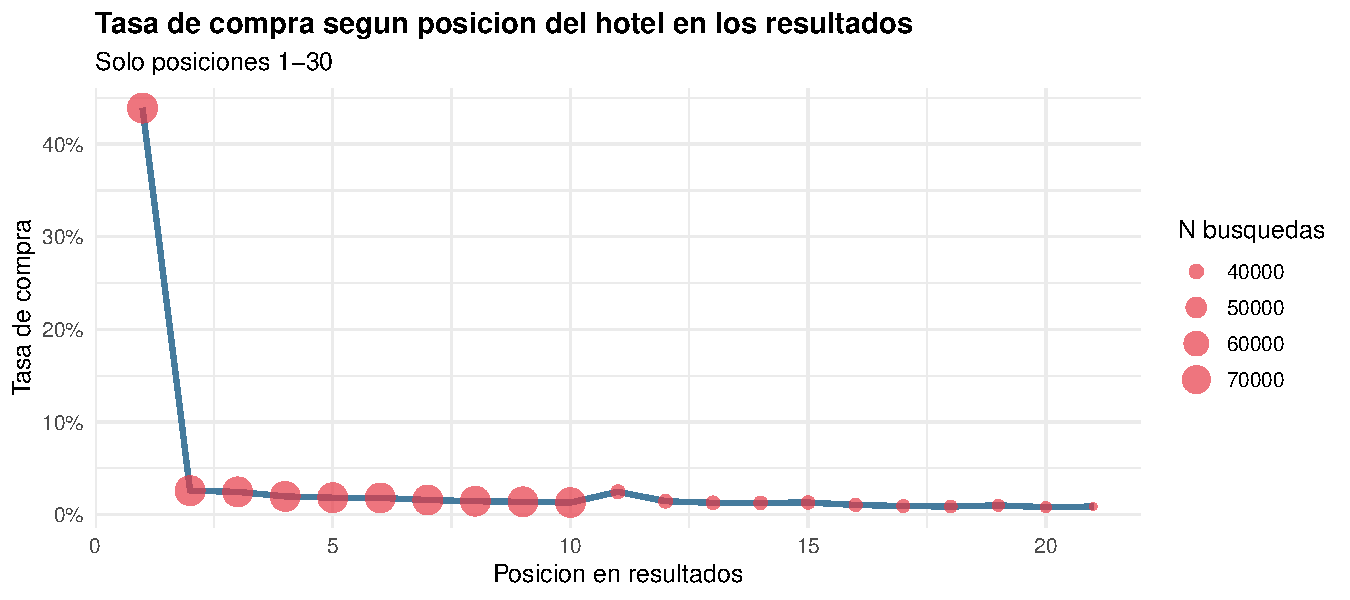
\includegraphics[width=\linewidth]{eda_posicion-1.pdf}
    \caption{Tasa de compra según posición en resultados.}
\end{figure}

\section{Ingeniería de Características}
Filtramos el dataset para abarcar exclusivamente Río de Janeiro (\texttt{geo\_id = 6381}) y definimos \texttt{price\_by\_night\_person} como variable objetivo (filtrando precios $\le 0$).

Se derivaron atributos temporales (día de la semana, fines de semana, feriados brasileños) y espaciales. Al cruzar el precio contra la distancia a Copacabana, la curva LOESS suavizada permite diagnosticar el gradiente espacial de valor.

\begin{figure}[htbp]
    \centering
    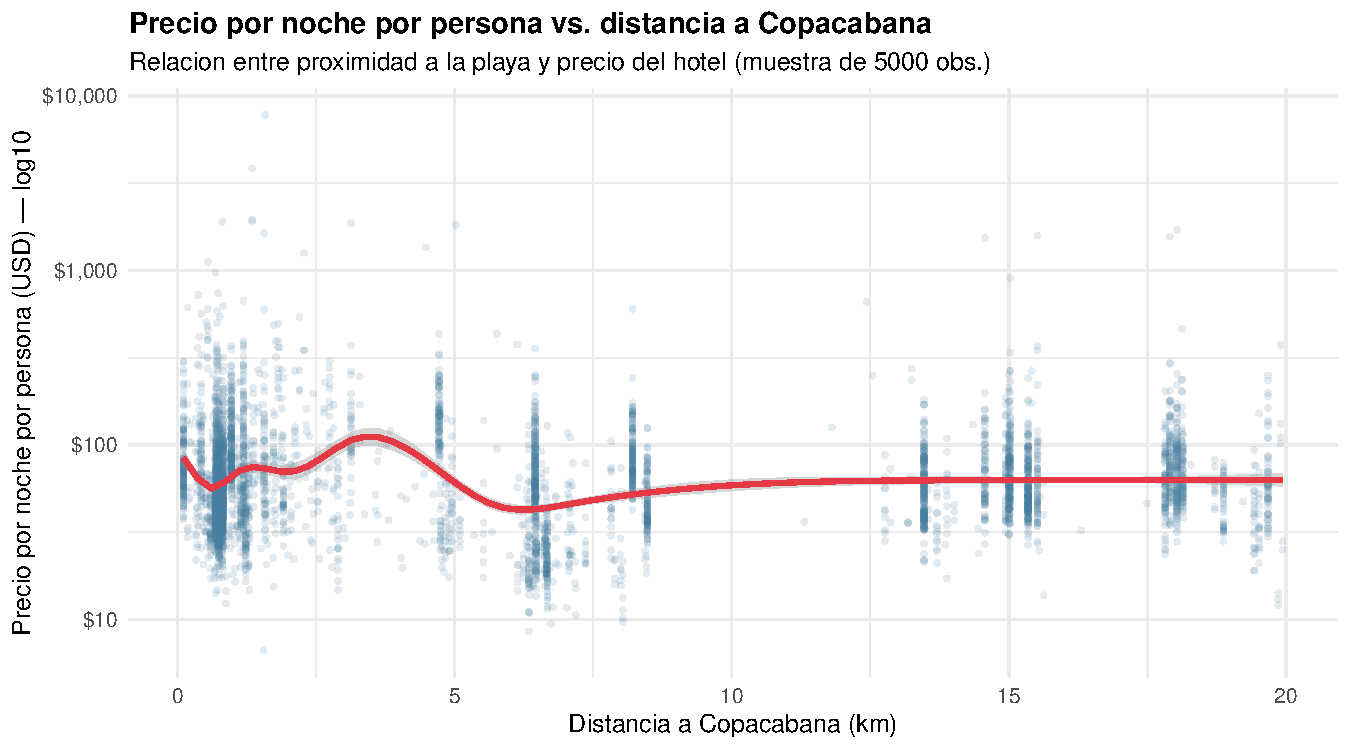
\includegraphics[width=\linewidth]{plot_dist_precio-1.pdf}
    \caption{Precio vs. Distancia a Copacabana con curva LOESS.}
\end{figure}

La relación exhibe una estructura no lineal: si bien la extrema varianza y los picos de precios máximos se aglomeran en las inmediaciones de la playa (distancias cercanas a 0 km), la caída tarifaria no es estrictamente monotónica. Esto evidencia la existencia de sub-centros urbanos de alto valor que imponen un premio de mercado independientemente de su lejanía con el epicentro de Copacabana. El tratamiento de valores anómalos se ejecutó aplicando un umbral restrictivo de $3 \times IQR$, y los valores faltantes en ratings se imputaron utilizando la mediana condicionada por categoría de estrellas.
\section{Modelado Predictivo}
A fin de aislar la inferencia de filtraciones futuras (Data Leakage), se removieron precios alternativos y el target. Se particionó la muestra en 80\% para entrenamiento y 20\% para validación cruzada.

\subsection{Baseline: Regresión Lineal Simple}
Se estableció un umbral utilizando \texttt{avgRating} ($r \approx 0.317$). El modelo univariado asume un crecimiento lineal tarifario.

\begin{figure}[htbp]
    \centering
    \includegraphics[width=\linewidth]{scatter_mejor_var.pdf}
    \caption{Regresión Lineal Baseline (Precio vs. avgRating).}
\end{figure}

La amplia dispersión de los residuos ($R^2 \approx 0.10$) certifica un severo sub-ajuste (underfitting), denotando que la tarifa no puede reducirse a un único vector paramétrico.

\subsection{Ensamble Arbóreo (Random Forest)}
Para capturar relaciones multivariadas no lineales, se entrenó un Random Forest mediante \texttt{ranger} (200 árboles, muestreo fraccionario del 30\%). 

\begin{figure}[htbp]
    \centering
    \includegraphics[width=\linewidth]{plot_reales_vs_pred-1.pdf}
    \caption{Predicciones vs. Valores Reales (Random Forest).}
\end{figure}

La nube de predicciones se alinea consistentemente con la bisectriz ideal, capturando aproximadamente el 45.1\% de la varianza natural y reduciendo los errores de magnitud significativamente frente a la línea base.

\subsection{Importancia de Variables (Feature Importance)}
La descomposición del incremento en el Error Cuadrático Medio por permutación revela los determinantes tarifarios.

\begin{figure}[htbp]
    \centering
    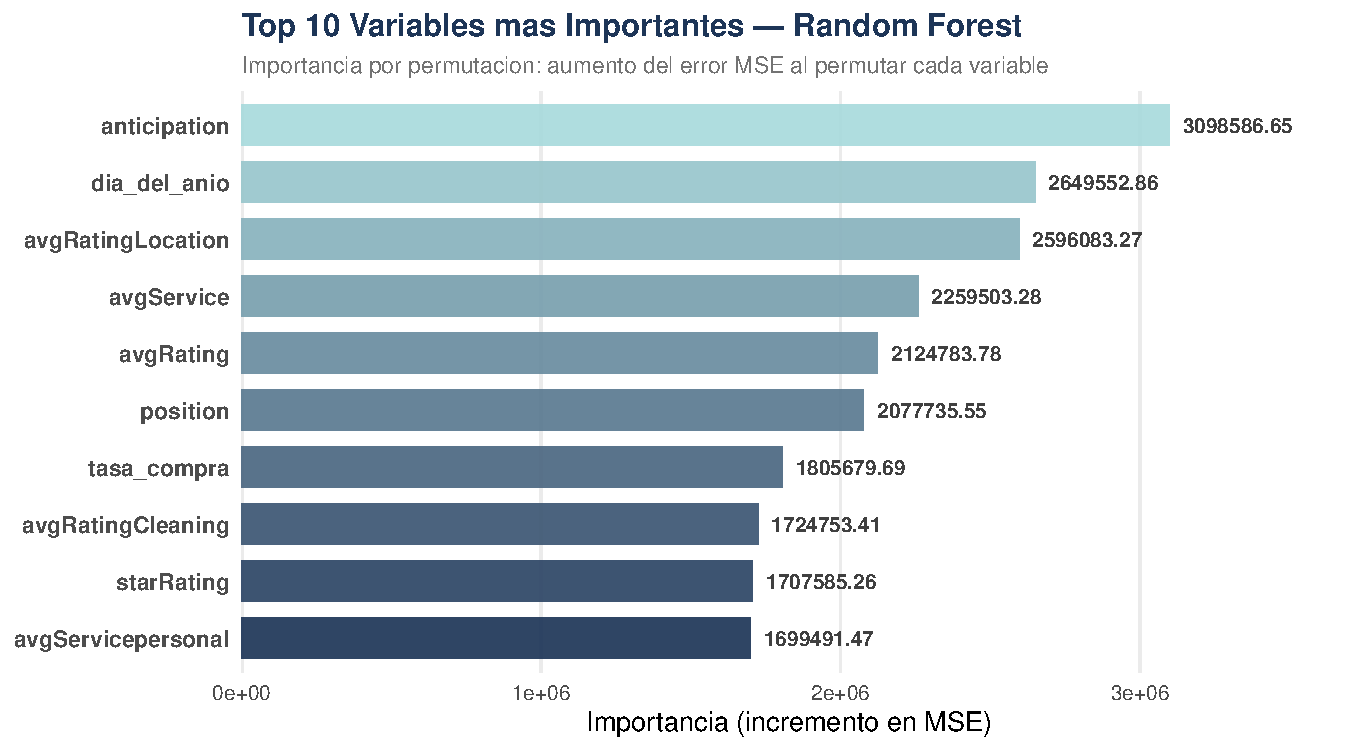
\includegraphics[width=\linewidth]{plot_feature_importance-1.pdf}
    \caption{Importancia Estructural de Variables (Top 10).}
\end{figure}

Los gradientes de urgencia (\texttt{anticipation}, \texttt{dia\_del\_anio}) y la centralidad del suelo (\texttt{avgRatingLocation}) tiranizan la estructura del precio, superando con creces a métricas de infraestructura física o ratings generales.

\section{Discusión y Conclusiones}
La síntesis computacional demuestra la ventaja innegable de la inferencia no paramétrica para decodificar la matriz tarifaria hotelera. Mientras los modelos lineales colapsan frente a la heterogeneidad del turismo, el algoritmo forestal multiplicó el poder explicativo.

A nivel metodológico, la técnica restrictiva de poda de outliers ($3 \times IQR$) garantizó estabilidad pero amputó la capacidad de predecir la cola pesada del segmento de hiper-lujo, requiriendo en el futuro abordajes especializados para distribuciones extremas. Pese a estas limitaciones, el modelo final constituye un artefacto robusto y analíticamente transparente para informar procesos de \textit{revenue management} en tiempo real.

\end{document}
